% Options for packages loaded elsewhere
\PassOptionsToPackage{unicode}{hyperref}
\PassOptionsToPackage{hyphens}{url}
%
\documentclass[
  10pt,
]{book}
\usepackage{lmodern}
\usepackage{amssymb,amsmath}
\usepackage{ifxetex,ifluatex}
\ifnum 0\ifxetex 1\fi\ifluatex 1\fi=0 % if pdftex
  \usepackage[T1]{fontenc}
  \usepackage[utf8]{inputenc}
  \usepackage{textcomp} % provide euro and other symbols
\else % if luatex or xetex
  \usepackage{unicode-math}
  \defaultfontfeatures{Scale=MatchLowercase}
  \defaultfontfeatures[\rmfamily]{Ligatures=TeX,Scale=1}
  \setmainfont[]{Liberation Serif}
  \setsansfont[]{Liberation Sans}
  \setmonofont[]{Liberation Mono}
\fi
% Use upquote if available, for straight quotes in verbatim environments
\IfFileExists{upquote.sty}{\usepackage{upquote}}{}
\IfFileExists{microtype.sty}{% use microtype if available
  \usepackage[]{microtype}
  \UseMicrotypeSet[protrusion]{basicmath} % disable protrusion for tt fonts
}{}
\makeatletter
\@ifundefined{KOMAClassName}{% if non-KOMA class
  \IfFileExists{parskip.sty}{%
    \usepackage{parskip}
  }{% else
    \setlength{\parindent}{0pt}
    \setlength{\parskip}{6pt plus 2pt minus 1pt}}
}{% if KOMA class
  \KOMAoptions{parskip=half}}
\makeatother
\usepackage{xcolor}
\IfFileExists{xurl.sty}{\usepackage{xurl}}{} % add URL line breaks if available
\IfFileExists{bookmark.sty}{\usepackage{bookmark}}{\usepackage{hyperref}}
\hypersetup{
  pdftitle={Utilisation du Markdown avec Pandoc},
  pdfauthor={Baptiste PIERARD},
  hidelinks,
  pdfcreator={LaTeX via pandoc}}
\urlstyle{same} % disable monospaced font for URLs
\usepackage[margin=2cm]{geometry}
\usepackage{color}
\usepackage{fancyvrb}
\newcommand{\VerbBar}{|}
\newcommand{\VERB}{\Verb[commandchars=\\\{\}]}
\DefineVerbatimEnvironment{Highlighting}{Verbatim}{commandchars=\\\{\}}
% Add ',fontsize=\small' for more characters per line
\newenvironment{Shaded}{}{}
\newcommand{\AlertTok}[1]{\textcolor[rgb]{1.00,0.00,0.00}{\textbf{#1}}}
\newcommand{\AnnotationTok}[1]{\textcolor[rgb]{0.38,0.63,0.69}{\textbf{\textit{#1}}}}
\newcommand{\AttributeTok}[1]{\textcolor[rgb]{0.49,0.56,0.16}{#1}}
\newcommand{\BaseNTok}[1]{\textcolor[rgb]{0.25,0.63,0.44}{#1}}
\newcommand{\BuiltInTok}[1]{#1}
\newcommand{\CharTok}[1]{\textcolor[rgb]{0.25,0.44,0.63}{#1}}
\newcommand{\CommentTok}[1]{\textcolor[rgb]{0.38,0.63,0.69}{\textit{#1}}}
\newcommand{\CommentVarTok}[1]{\textcolor[rgb]{0.38,0.63,0.69}{\textbf{\textit{#1}}}}
\newcommand{\ConstantTok}[1]{\textcolor[rgb]{0.53,0.00,0.00}{#1}}
\newcommand{\ControlFlowTok}[1]{\textcolor[rgb]{0.00,0.44,0.13}{\textbf{#1}}}
\newcommand{\DataTypeTok}[1]{\textcolor[rgb]{0.56,0.13,0.00}{#1}}
\newcommand{\DecValTok}[1]{\textcolor[rgb]{0.25,0.63,0.44}{#1}}
\newcommand{\DocumentationTok}[1]{\textcolor[rgb]{0.73,0.13,0.13}{\textit{#1}}}
\newcommand{\ErrorTok}[1]{\textcolor[rgb]{1.00,0.00,0.00}{\textbf{#1}}}
\newcommand{\ExtensionTok}[1]{#1}
\newcommand{\FloatTok}[1]{\textcolor[rgb]{0.25,0.63,0.44}{#1}}
\newcommand{\FunctionTok}[1]{\textcolor[rgb]{0.02,0.16,0.49}{#1}}
\newcommand{\ImportTok}[1]{#1}
\newcommand{\InformationTok}[1]{\textcolor[rgb]{0.38,0.63,0.69}{\textbf{\textit{#1}}}}
\newcommand{\KeywordTok}[1]{\textcolor[rgb]{0.00,0.44,0.13}{\textbf{#1}}}
\newcommand{\NormalTok}[1]{#1}
\newcommand{\OperatorTok}[1]{\textcolor[rgb]{0.40,0.40,0.40}{#1}}
\newcommand{\OtherTok}[1]{\textcolor[rgb]{0.00,0.44,0.13}{#1}}
\newcommand{\PreprocessorTok}[1]{\textcolor[rgb]{0.74,0.48,0.00}{#1}}
\newcommand{\RegionMarkerTok}[1]{#1}
\newcommand{\SpecialCharTok}[1]{\textcolor[rgb]{0.25,0.44,0.63}{#1}}
\newcommand{\SpecialStringTok}[1]{\textcolor[rgb]{0.73,0.40,0.53}{#1}}
\newcommand{\StringTok}[1]{\textcolor[rgb]{0.25,0.44,0.63}{#1}}
\newcommand{\VariableTok}[1]{\textcolor[rgb]{0.10,0.09,0.49}{#1}}
\newcommand{\VerbatimStringTok}[1]{\textcolor[rgb]{0.25,0.44,0.63}{#1}}
\newcommand{\WarningTok}[1]{\textcolor[rgb]{0.38,0.63,0.69}{\textbf{\textit{#1}}}}
\usepackage{longtable,booktabs}
% Correct order of tables after \paragraph or \subparagraph
\usepackage{etoolbox}
\makeatletter
\patchcmd\longtable{\par}{\if@noskipsec\mbox{}\fi\par}{}{}
\makeatother
% Allow footnotes in longtable head/foot
\IfFileExists{footnotehyper.sty}{\usepackage{footnotehyper}}{\usepackage{footnote}}
\makesavenoteenv{longtable}
\usepackage{graphicx}
\makeatletter
\def\maxwidth{\ifdim\Gin@nat@width>\linewidth\linewidth\else\Gin@nat@width\fi}
\def\maxheight{\ifdim\Gin@nat@height>\textheight\textheight\else\Gin@nat@height\fi}
\makeatother
% Scale images if necessary, so that they will not overflow the page
% margins by default, and it is still possible to overwrite the defaults
% using explicit options in \includegraphics[width, height, ...]{}
\setkeys{Gin}{width=\maxwidth,height=\maxheight,keepaspectratio}
% Set default figure placement to htbp
\makeatletter
\def\fps@figure{htbp}
\makeatother
\setlength{\emergencystretch}{3em} % prevent overfull lines
\providecommand{\tightlist}{%
  \setlength{\itemsep}{0pt}\setlength{\parskip}{0pt}}
\setcounter{secnumdepth}{5}

\title{Utilisation du Markdown avec Pandoc}
\author{Baptiste PIERARD}
\date{21 avril 2020}

\begin{document}
\frontmatter
\maketitle

{
\setcounter{tocdepth}{2}
\tableofcontents
}
\mainmatter
\hypertarget{introduction}{%
\section{INTRODUCTION}\label{introduction}}

\hypertarget{but-responsabilituxe9s-domaine-dapplication}{%
\subsection{But, Responsabilités, Domaine
d'application}\label{but-responsabilituxe9s-domaine-dapplication}}

\hypertarget{objectifs}{%
\subsubsection{Objectifs}\label{objectifs}}

Ce paragraphe donne la raison d'être du document. Il s'articule de la
manière suivante :

\begin{itemize}
\tightlist
\item
  But du système dans une description rapide.
\item
  But du Sous-Système dans une description rapide.
\item
  But du document.
\end{itemize}

Cette description de quelques lignes apparaîtra dans tous les documents
relatifs au sous-système. Il est conseillé de recopier mot pour mot
cette description sur l'ensemble des documents.

\hypertarget{responsabilituxe9s}{%
\subsubsection{Responsabilités}\label{responsabilituxe9s}}

Ce paragraphe donne les responsabilités associées au document, notamment
:

\begin{itemize}
\tightlist
\item
  le nom de l'auteur ou de l'équipe de rédaction,
\item
  le nom du vérificateur,
\item
  le nom de celui qui approuve le document.
\end{itemize}

Si ces informations sont déjà données dans le Plan Qualité du projet, il
faut l'indiquer par la phrase suivante :

Les responsabilités associées à ce document sont définies dans le Plan
Qualité du Projet.

\hypertarget{domaine-dapplication}{%
\subsubsection{Domaine d'application}\label{domaine-dapplication}}

Ce paragraphe précise à quel sous-ensemble du projet correspond ce
document, et à quelle version du ou des composants. Par exemple s'il
s'agit d'un logiciel :

Ce document correspond à la version VXXX.Y du logiciel\ldots{}

\hypertarget{hypothuxe8ses}{%
\subsection{Hypothèses}\label{hypothuxe8ses}}

Ce paragraphe décrit les hypothèses utilisées pour la rédaction. Les
parties en italiques dans ce modèle sont des guides de rédactions.

\hypertarget{documents-applicables-de-ruxe9fuxe9rence}{%
\subsection{Documents applicables, de
référence}\label{documents-applicables-de-ruxe9fuxe9rence}}

Ces paragraphes donnent la liste des documents d'entrée de ce document.

\hypertarget{documents-muxe9diane-systuxe8me-applicables}{%
\subsubsection{Documents Médiane Système
applicables}\label{documents-muxe9diane-systuxe8me-applicables}}

Doivent au moins apparaître

\begin{itemize}
\tightlist
\item
  le Manuel Qualité de Médiane Système,
\item
  le Plan Qualité du projet puis,
\item
  la Spécification si ce document est une Conception,
\item
  et ainsi de suite\ldots{}
\end{itemize}

\begin{longtable}[]{@{}cllcc@{}}
\caption{Documents applicables.}\tabularnewline
\toprule
Abréviation & Nom du document & Description et/ou titre & Version &
Date\tabularnewline
\midrule
\endfirsthead
\toprule
Abréviation & Nom du document & Description et/ou titre & Version &
Date\tabularnewline
\midrule
\endhead
{[}MQE{]} & SysQ\_MQE\_N.n.DOC & Manuel Qualité et Environnement & 1.0 &
jj/mm/aaaa\tabularnewline
{[}PQP{]} & AAAA\_PQP\_N.n.DOC & Plan Qualité Projet & 2.0 &
jj/mm/aaaa\tabularnewline
\bottomrule
\end{longtable}

\hypertarget{documents-externes-applicables}{%
\subsubsection{Documents externes
applicables}\label{documents-externes-applicables}}

Peuvent apparaître :

\begin{itemize}
\tightlist
\item
  le Cahier des charges si ce document est une Spécification,
\item
  des spécifications client,
\item
  et ainsi de suite\ldots{}
\end{itemize}

\begin{longtable}[]{@{}cllcc@{}}
\caption{Documents exernes applicables.}\tabularnewline
\toprule
Abréviation & Nom du document & Description et/ou titre & Version &
Date\tabularnewline
\midrule
\endfirsthead
\toprule
Abréviation & Nom du document & Description et/ou titre & Version &
Date\tabularnewline
\midrule
\endhead
{[}CdC{]} & CdC\_Projet\_Toto & Cahier Des Charges & 1.0a &
jj/mm/aaaa\tabularnewline
\bottomrule
\end{longtable}

\hypertarget{documents-de-ruxe9fuxe9rence}{%
\subsubsection{Documents de
référence}\label{documents-de-ruxe9fuxe9rence}}

Un document de référence est un document utilisé pour la rédaction de
cette spécification :

\begin{itemize}
\tightlist
\item
  guide de rédaction,
\item
  manuel utilisateur d'un logiciel,
\item
  règlements
\item
  etc\ldots{}
\end{itemize}

Les documents cités doivent être identifiés de la même manière que pour
les documents applicables.

\begin{longtable}[]{@{}cllcc@{}}
\caption{Identification des documents.}\tabularnewline
\toprule
Notation abrégée & Titre & Référence & Version & Date\tabularnewline
\midrule
\endfirsthead
\toprule
Notation abrégée & Titre & Référence & Version & Date\tabularnewline
\midrule
\endhead
RdC & Règles de Codage C & ??? & 1.0 & jj/mm/aaaa\tabularnewline
\bottomrule
\end{longtable}

\hypertarget{terminologie}{%
\subsection{Terminologie}\label{terminologie}}

Ce paragraphe permet au lecteur néophyte de se débrouiller dans la
jungle des sigles et symboles du projet\ldots{} Ne pas hésiter à
renvoyer à un document donnant une définition exacte des sigles ou noms
les plus importants.

\begin{longtable}[]{@{}ll@{}}
\toprule
\begin{minipage}[b]{0.23\columnwidth}\raggedright
Terme ou symbole\strut
\end{minipage} & \begin{minipage}[b]{0.71\columnwidth}\raggedright
Correspondance\strut
\end{minipage}\tabularnewline
\midrule
\endhead
\begin{minipage}[t]{0.23\columnwidth}\raggedright
\textbf{RTFM}\strut
\end{minipage} & \begin{minipage}[t]{0.71\columnwidth}\raggedright
\textbf{R}ead \textbf{T}he \textbf{F}ile \textbf{M}anual

Ayez l'obligeance de vous reporter au manuel utilisateur\strut
\end{minipage}\tabularnewline
\begin{minipage}[t]{0.23\columnwidth}\raggedright
\textbf{PDJ}\strut
\end{minipage} & \begin{minipage}[t]{0.71\columnwidth}\raggedright
\textbf{P}etit \textbf{D}é\textbf{J}euner

Repas le plus important de la journée\strut
\end{minipage}\tabularnewline
\bottomrule
\end{longtable}

\hypertarget{contenu-du-document}{%
\section{CONTENU DU DOCUMENT\ldots{}}\label{contenu-du-document}}

Ce document présente l'architecture générale du logicel :

\begin{figure}
\centering
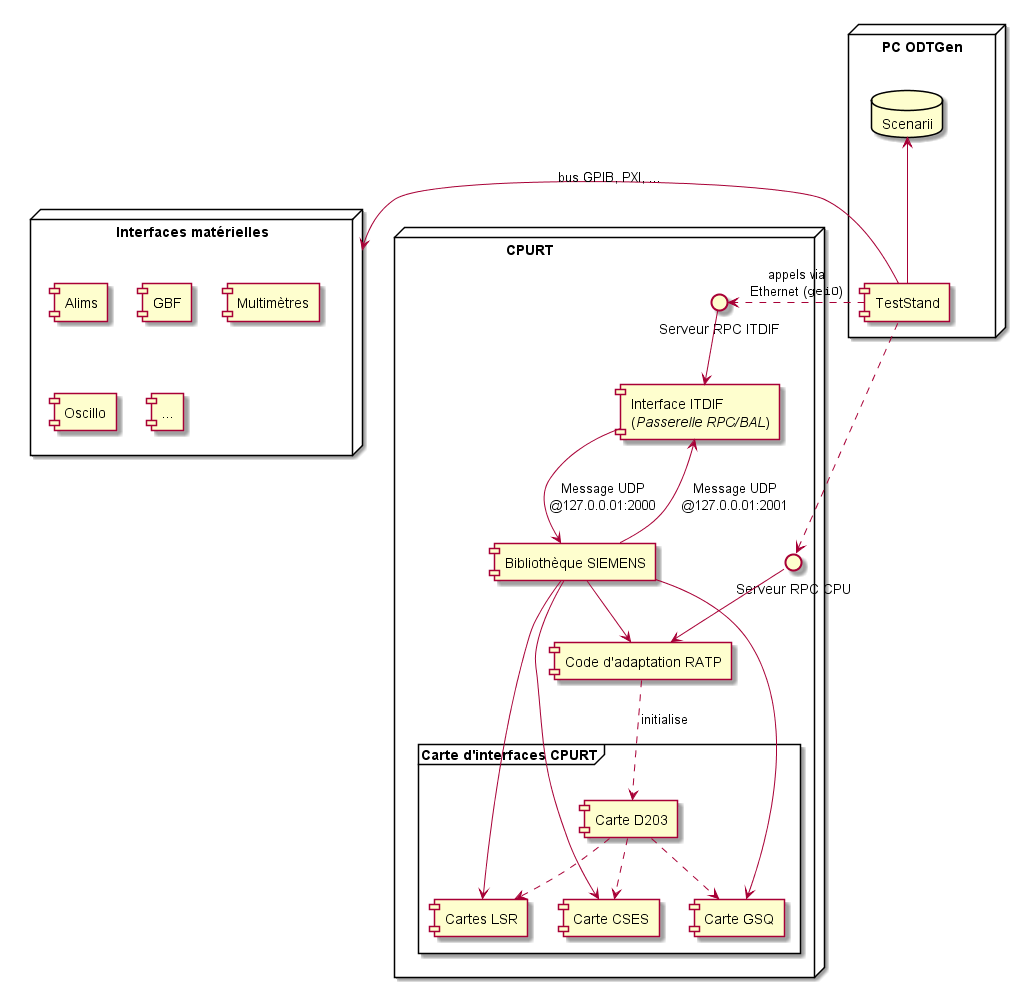
\includegraphics{./tex2pdf.-1f50f5654d7493c4/ae1a89740bab541d6c24e90760040d81d9c06d87.png}
\caption{Figure 1 : Composants principaux du projet}
\end{figure}

Voici un diagramme de séquences entièrement rédigé en mode texe :

\begin{figure}
\centering
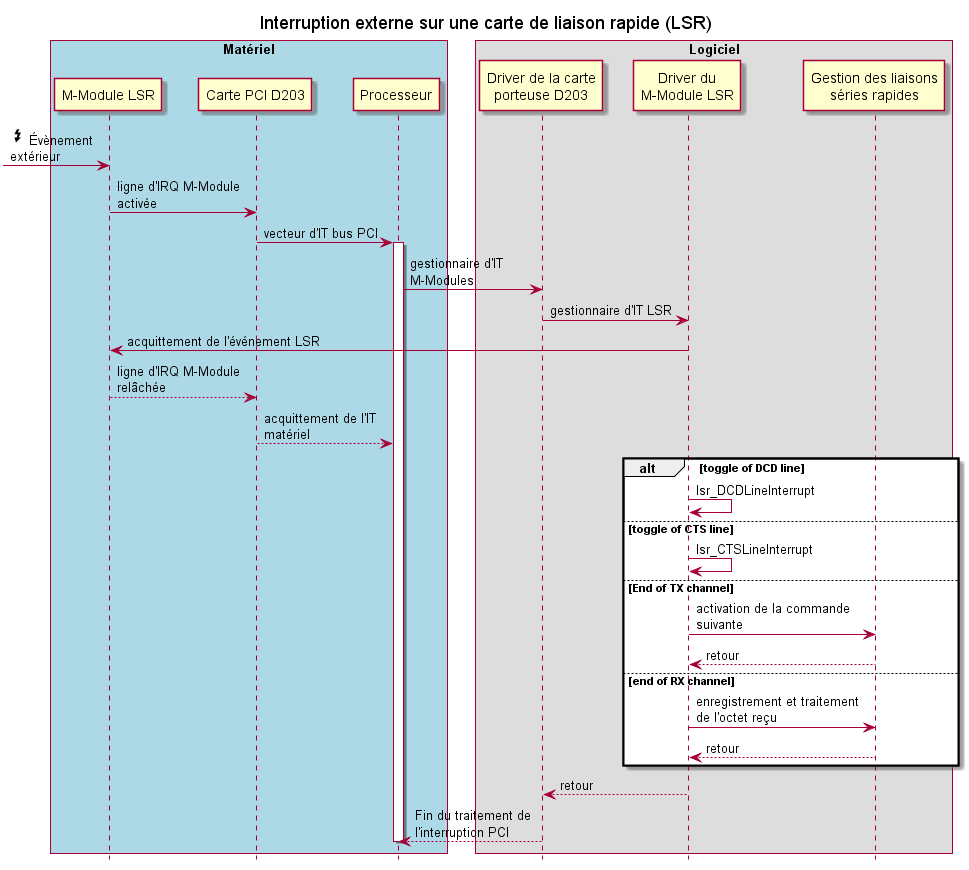
\includegraphics{./tex2pdf.-1f50f5654d7493c4/45ba3739ec0b86aa812dc13714ec55161459beee.png}
\caption{Figure 2 : Diagramme de séquence PlantUML}
\end{figure}

\hypertarget{titre-de-niveau-1}{%
\section{Titre de niveau 1}\label{titre-de-niveau-1}}

\hypertarget{titre-de-niveau-2}{%
\subsection{Titre de niveau 2}\label{titre-de-niveau-2}}

\hypertarget{titre-de-niveau-3}{%
\subsubsection{Titre de niveau 3}\label{titre-de-niveau-3}}

ceci est un paragraphe.

Lorem ipsum dolor sit amet, consectetur adipiscing elit. Sed vitae nunc
vitae nulla feugiat tempor eu vitae lacus. Vestibulum malesuada
consequat magna at eleifend. In hac habitasse platea dictumst. Cras
placerat molestie sem non feugiat. Etiam sit amet metus vel ligula
egestas laoreet non sit amet lacus. Praesent quis quam non augue
pellentesque placerat. Sed et leo id odio imperdiet tempor. In dapibus
elit in mauris hendrerit dictum. Donec quis nibh eu ipsum auctor varius.
Pellentesque quis scelerisque tellus. Etiam a augue nulla. Nam placerat
mi ac massa mattis, nec vehicula diam interdum. Aliquam erat volutpat.
Ut eu tempor risus.

Phasellus rutrum vehicula sapien, ut maximus felis. Mauris blandit
lectus convallis tellus porta varius. Vestibulum et aliquam felis, at
semper ex. Etiam convallis urna sit amet pulvinar finibus. Duis bibendum
metus congue ex eleifend, ac consectetur diam lobortis. Aliquam
porttitor leo diam, ac tempus odio semper a. Nullam eu imperdiet metus.
Nunc sem ligula, finibus non metus eu, congue consequat eros. Integer
mattis pulvinar consectetur. Phasellus eget augue sit amet nibh iaculis
sagittis. Aenean sed nisl nec libero semper dignissim. Fusce a urna
bibendum, pharetra leo viverra, tristique urna. Nullam felis neque,
faucibus sit amet mi ac, hendrerit euismod orci. Nulla facilisi. Morbi
tristique tempus risus. Vestibulum finibus risus arcu, non tempus risus
vehicula eget.

Suspendisse scelerisque mollis libero, eu maximus enim interdum a. Fusce
congue, nisl et tristique ullamcorper, libero sapien tincidunt risus,
vel gravida nunc elit eget magna. In hac habitasse platea dictumst.
Praesent nec est sit amet nunc mollis accumsan vitae sit amet massa.
Proin et ligula a magna laoreet consectetur. Nullam iaculis leo in urna
efficitur, sed tincidunt tellus mollis. Fusce feugiat auctor urna sed
fermentum.

\hypertarget{titre-de-niveau-3-1}{%
\subsubsection{Titre de niveau 3}\label{titre-de-niveau-3-1}}

Et voila un exemple de liste non-numérotée :

\begin{itemize}
\tightlist
\item
  pomme
\item
  poire
\item
  carotte
\item
  navet
\end{itemize}

Voici un exemple de liste numérotée :

\begin{enumerate}
\def\labelenumi{\arabic{enumi}.}
\tightlist
\item
  Tintin
\item
  Milou
\item
  Haddock
\end{enumerate}

Et un exemple de \emph{todo list} (cases à cocher) :

\begin{itemize}
\tightlist
\item[$\square$]
  non coché
\item[$\boxtimes$]
  coché
\end{itemize}

\hypertarget{titre-de-niveau-3-2}{%
\subsubsection{Titre de niveau 3}\label{titre-de-niveau-3-2}}

Lorem ipsum dolor sit amet, consectetur adipiscing elit. Sed vitae nunc
vitae nulla feugiat tempor eu vitae lacus. Vestibulum malesuada
consequat magna at eleifend. In hac habitasse platea dictumst. Cras
placerat molestie sem non feugiat. Etiam sit amet metus vel ligula
egestas laoreet non sit amet lacus. Praesent quis quam non augue
pellentesque placerat. Sed et leo id odio imperdiet tempor. In dapibus
elit in mauris hendrerit dictum. Donec quis nibh eu ipsum auctor varius.
Pellentesque quis scelerisque tellus. Etiam a augue nulla. Nam placerat
mi ac massa mattis, nec vehicula diam interdum. Aliquam erat volutpat.
Ut eu tempor risus.

\begin{quote}
Ceci est une citation : « C'est curieux chez les marins ce besoin de
faire des phrases ! »
\end{quote}

\hypertarget{autre-titre-de-niveau-2}{%
\subsection{Autre titre de niveau 2}\label{autre-titre-de-niveau-2}}

Ce fichier \texttt{.md} est encodé en UTF8, pour ne pas avoir de
problème lors de l'utilisation de caractères accentués ou spéciaux.

Exemple de code source en C :

\begin{Shaded}
\begin{Highlighting}[]
\PreprocessorTok{\#include }\ImportTok{"triangle.h"}
\PreprocessorTok{\#include }\ImportTok{<math.h>}

\CommentTok{//====================================================================}
\CommentTok{// Determination du type d\textquotesingle{}un triangle}
\CommentTok{//====================================================================}
\DataTypeTok{char}\NormalTok{* QualifierTriangle(}\DataTypeTok{unsigned} \DataTypeTok{int}\NormalTok{ a, }\DataTypeTok{unsigned} \DataTypeTok{int}\NormalTok{ b, }\DataTypeTok{unsigned} \DataTypeTok{int}\NormalTok{ c)}
\NormalTok{\{}
    \ControlFlowTok{if}\NormalTok{( a+b<=c || b+c<=a || c+a<=b )}
\NormalTok{    \{}
        \ControlFlowTok{return} \StringTok{"impossible"}\NormalTok{;}
\NormalTok{    \}}
    \ControlFlowTok{else}
\NormalTok{    \{}
        \DataTypeTok{unsigned} \DataTypeTok{int}\NormalTok{ egalite=}\DecValTok{0}\NormalTok{;}
        \ControlFlowTok{if}\NormalTok{ (a==b) egalite++;}
        \ControlFlowTok{if}\NormalTok{ (a==c) egalite++;}
        \ControlFlowTok{if}\NormalTok{ (c==b) egalite++;}

        \ControlFlowTok{if}\NormalTok{ (egalite==}\DecValTok{0}\NormalTok{)      }\ControlFlowTok{return} \StringTok{"quelconque"}\NormalTok{;}
        \ControlFlowTok{else} \ControlFlowTok{if}\NormalTok{ (egalite==}\DecValTok{1}\NormalTok{) }\ControlFlowTok{return} \StringTok{"isocele"}\NormalTok{;}
        \ControlFlowTok{else}                 \ControlFlowTok{return} \StringTok{"equilateral"}\NormalTok{;}
\NormalTok{    \}}
\NormalTok{\}}
\end{Highlighting}
\end{Shaded}

avec le logigramme associé, rédigé en mode texte, et traité par le
logiciel PlantUML pour en générer une image :

\begin{figure}
\centering
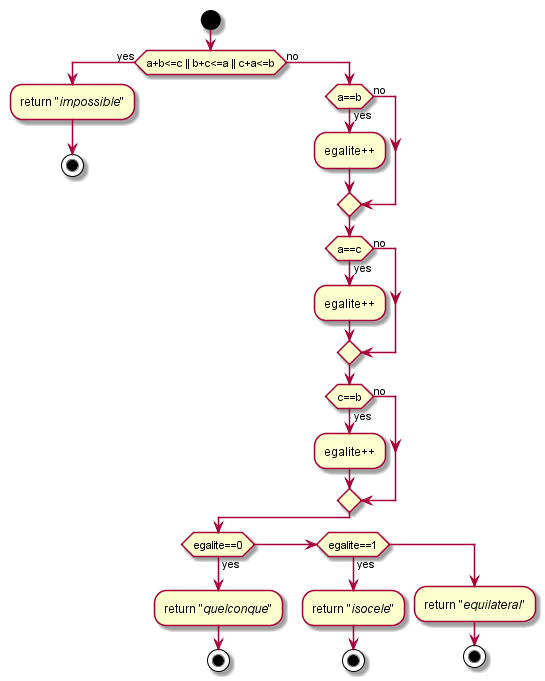
\includegraphics{./tex2pdf.-1f50f5654d7493c4/236c15226c43ff9726a0f782e89309124a2f03cb.png}
\caption{Figure 3 : Logigramme de qualification d'un triangle}
\end{figure}

ou bien en java

\begin{Shaded}
\begin{Highlighting}[]
\KeywordTok{public} \KeywordTok{class}\NormalTok{ HelloWorld \{}

    \KeywordTok{public} \DataTypeTok{static} \DataTypeTok{void} \FunctionTok{main}\NormalTok{(}\BuiltInTok{String}\NormalTok{[] args) \{}
        \BuiltInTok{System}\NormalTok{.}\FunctionTok{out}\NormalTok{.}\FunctionTok{println}\NormalTok{(}\StringTok{"Hello, World"}\NormalTok{);}
\NormalTok{    \}}

\NormalTok{\}}
\end{Highlighting}
\end{Shaded}

ou bien en python (\emph{on appréciera au passage la concision du
language par rapport au java !}) :

\begin{Shaded}
\begin{Highlighting}[]
\BuiltInTok{print} \StringTok{"Hello World"}
\end{Highlighting}
\end{Shaded}

Exemple de diagrammes de temps généré à l'aide de PlantUML :

\begin{figure}
\centering
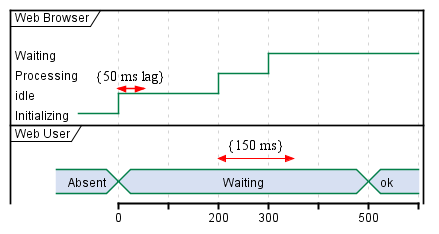
\includegraphics{./tex2pdf.-1f50f5654d7493c4/3351154ec6feb4aecc4c725551dd76f7f033eea2.png}
\caption{Figure 4 : Diagramme de temps : Affichage d'une page Web}
\end{figure}

Exemples de diagrammes de Gantt générés à l'aide de PlantUML :

\begin{figure}
\centering
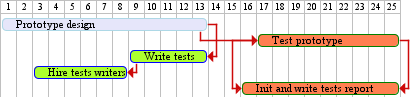
\includegraphics{./tex2pdf.-1f50f5654d7493c4/51a23f36ae650b0334f0669a62cba3804f07b496.png}
\caption{Figure 5 : Diagramme de Gantt}
\end{figure}

\begin{figure}
\centering
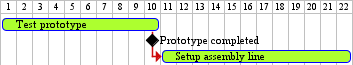
\includegraphics{./tex2pdf.-1f50f5654d7493c4/923da1012067e6567c647e5d67f74b2dda84906a.png}
\caption{Figure 6 : Diagramme de Gantt}
\end{figure}

\begin{figure}
\centering
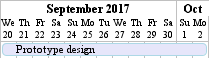
\includegraphics{./tex2pdf.-1f50f5654d7493c4/cbe3c882ef3665a2ee8c9a5bb5d0327823462fe2.png}
\caption{Figure 7 : Diagramme de Gantt}
\end{figure}

\hypertarget{notations-mathuxe9matiques}{%
\subsection{Notations mathématiques}\label{notations-mathuxe9matiques}}

Exemple de notation mathématique, en mettant le texte entre deux dollars
:

\begin{itemize}
\tightlist
\item
  \(1 + 1 = 2\)
\item
  \(\sqrt{\frac{x^2}{3}}\)
\item
  \(x_{1,2} = \frac{- b \pm \sqrt{\Delta}}{2a}\)
\item
  \(\begin{bmatrix}  a_1 & b_1 \\  a_2 & b_2 \end{bmatrix}\)
\item
  \(\sum_{x=0}^n f(x)\)
\end{itemize}

\hypertarget{diagrammes-divers}{%
\subsection{Diagrammes divers}\label{diagrammes-divers}}

Example usage:

\begin{figure}
\centering
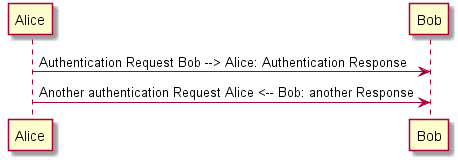
\includegraphics{./tex2pdf.-1f50f5654d7493c4/9824b34cea484ebda9342f4f8056531c58f33557.png}
\caption{This is an image, created by \textbf{PlantUML}.}
\end{figure}

\hypertarget{graphviz}{%
\subsubsection{Graphviz}\label{graphviz}}

To use Graphviz you only need to install Graphviz, as you can read on
its \href{http://www.graphviz.org/}{website}. There are no other
dependencies.

This filter assumes that the \texttt{dot} command is located in the path
and therefore can be used from any location. Alternatively, you can set
the environment variable \texttt{DOT} or use the pandoc's meta variable
\texttt{dotPath}.

Example usage from
\href{https://graphviz.gitlab.io/_pages/Gallery/directed/fsm.html}{the
Graphviz gallery}:

\begin{figure}
\centering
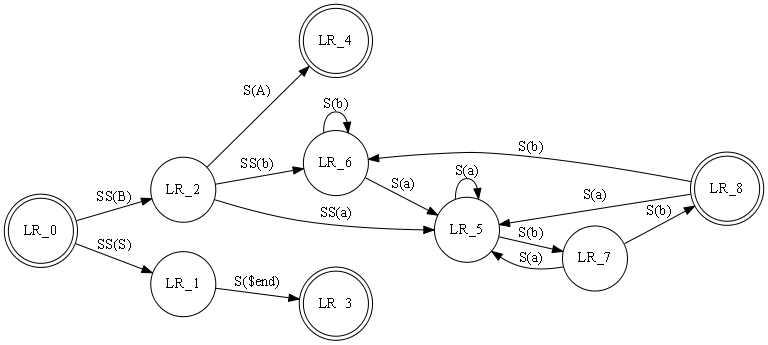
\includegraphics{./tex2pdf.-1f50f5654d7493c4/41a1b7e18b45d94e590ef40ebcf3e52f86f470d1.png}
\caption{This is an image, created by \textbf{Graphviz}'s dot.}
\end{figure}

\backmatter
\end{document}
